% This document show you how to draw a scalebar onto a figure. If you want to
% draw a scale-bar and you don't really know the length, take a look at
% 'scalebar.tex' in this repository, which also shows you how to calculate the
% length, depending on the image.

\documentclass{article}
\usepackage{graphicx}
\usepackage{tikz}
	\usetikzlibrary{shapes.arrows}
\usepackage{siunitx}
\usepackage[graphics,tightpage,active]{preview}
\PreviewEnvironment{tikzpicture}

\newcommand{\imsize}{\linewidth}
\newlength\imagewidth
\newlength\imagescale

\begin{document}
	\pgfmathsetlength{\imagewidth}{\linewidth} % desired displayed width of image
	\pgfmathsetlength{\imagescale}{\imagewidth/670} % pixel width of imagefile used below
 
	% adjust scale of tikzpicture (and direction of y) such that pixel
	% coordinates can be used for drawing overlays:
	\begin{tikzpicture}[x=\imagescale,y=-\imagescale]
		% place image (integer coordinates refer to pixel centers):
		\node[anchor=north west,inner sep=0pt,outer sep=0pt] at (0,0) {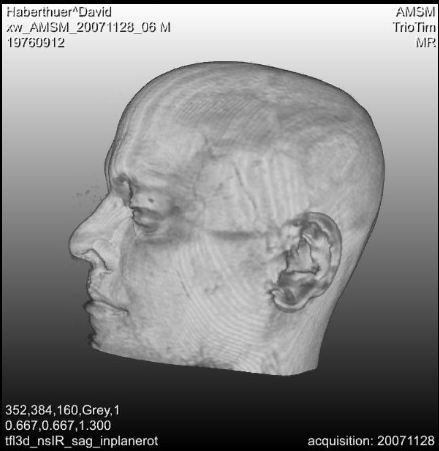
\includegraphics[width=\imagewidth]{scalebarimage}};
		\draw[|-|,red,ultra thick] (25,500) -- (175,500) node [midway,above] {\SI{300}{\micro\meter}}; % coordinates where the scalebar should be drawn, scaled with the size of the image.
	\end{tikzpicture}
\end{document}
